\documentclass{article}
\usepackage{graphicx}
\usepackage{listings}
\usepackage{xcolor}
\usepackage{amsmath}
\usepackage{float}
\usepackage{booktabs} 
\usepackage{geometry}
\usepackage{mathptmx} % 论文中常用的学术级字体 (Times New Roman风格)

\geometry{a4paper, margin=1in}

% 定义与Python自带编辑器(IDLE)一致的代码高亮颜色
\definecolor{idlekeyword}{HTML}{FF7700} % 关键字：橙色
\definecolor{idlestring}{HTML}{00AA00}  % 字符串：绿色
\definecolor{idlecomment}{HTML}{DD0000} % 注释：红色

\lstset{
	language=Python,
	basicstyle=\ttfamily\footnotesize,
	keywordstyle=\color{idlekeyword}\bfseries,
	stringstyle=\color{idlestring},
	commentstyle=\color{idlecomment},
	breaklines=true,
	frame=single,
	showstringspaces=false
}

\title{Research on photovoltaic power generation based on multi-dimensional indicators and models}
\author{Pengying Fan, Zhenlin Chen and Yile Wang}
\date{}

\begin{document}
	\maketitle
	
	\section{Introduction}
	As one of the world's largest energy consumers, China's power supply system is crucial to the stability of its domestic economy and society. In recent years, with the rapid economic development and the advancement of industrialization and urbanization, the demand for electricity has continued to grow, and higher requirements have been placed on power generation supply (Nie et al., 2024). At present, the power generation structure in China is diversified. Traditional energy generation, especially coal power generation, still dominates because of its abundant reserves and low price, but it brings serious environmental problems and faces environmental protection pressure (Zheng et al., 2025). Meanwhile, the Chinese government is actively developing renewable energy sources such as solar and wind power, among which photovoltaic power generation has made significant progress. China has become one of the largest photovoltaic markets in the world, with power stations all over the country, especially in the western region. The growth in photovoltaic power helps reduce reliance on traditional energy sources and supports carbon reduction targets. However, photovoltaic power faces challenges such as being greatly affected by the weather, stability and reliability need to be addressed, and high construction and operation costs require technological innovation and policy support to reduce costs and address environmental issues (Rahman et al., 2025). In addition, China's power supply is unevenly distributed across regions, with high demand but scarce resources in the eastern coastal areas and abundant resources but low demand in the western regions. Therefore, strengthening the construction of power transmission and distribution networks and achieving cross-regional interconnection are important ways to solve the contradiction between regional power supply and demand. In conclusion, China's power supply system is facing an important period of transition from traditional energy to clean energy. Although coal power generation still dominates, the rapid development of renewable energy such as photovoltaic power generation brings new hope for future power supply. The government needs to continue to increase policy support, promote technological innovation and market development to achieve sustainable development of power supply and green transformation of the economy and society.
	
	\section{Literature review}
	Photovoltaic (PV) power generation, as an important clean energy source, has gained widespread attention globally in recent years. Despite continuous technological advancements, PV power generation still faces several challenges, such as poor stability, high costs, and environmental impacts. Existing research has explored various aspects of PV power generation, including efficiency, economic viability, and carbon emissions, but numerous challenges remain to be addressed, particularly in improving power generation efficiency, reducing costs, and mitigating carbon emissions. In addition, regional differences in electricity demand and resource distribution, as well as the policy and market environment, have also had a significant impact on the development of PV power generation. In the following sections, we will review the relevant literature, analyze the limitations of existing research, and discuss potential future research directions.
	
	\subsection{Development of multi-dimensional indicator systems for photovoltaic power generation}
	In photovoltaic (PV) power generation research, an increasing number of scholars have recognized that relying solely on indicators such as "power generation efficiency" or "economic viability" cannot comprehensively assess the sustainability and application potential of PV systems (Liu J. et al., 2025). Early studies incorporated metrics such as energy payback time (Barbosa, 2026), return on investment (Lei et al., 2025), greenhouse gas emission intensity (Xu et al., 2025), and net present value (Ellis et al., 2023) into a unified evaluation framework, thereby enabling the comprehensive ranking of different PV system options. Furthermore, some research has developed a comprehensive evaluation system for the feasibility of PV projects (Djalab et al., 2024), which considers factors such as technology type (Si et al., 2024), cost (Chong et al., 2024), environmental impact (Si et al., 2024), and policy support (Chong et al., 2023). With the advancement of Geographic Information Systems (GIS) and remote sensing technologies, an increasing number of studies have introduced spatial dimensions into site selection and potential assessment (Lambarki et al., 2025), incorporating metrics such as solar radiation (Yao et al., 2024), land use (Sanda et al., 2026), and slope/aspect (Dhivagar et al., 2025) into evaluation systems. This enables the provision of reasonable layout recommendations for both centralized and distributed PV systems. Some studies have attempted to integrate the "lifecycle terminal management" of PV systems into multidimensional evaluation methods (Liu H. et al., 2025). For instance, Hernández-López et al. (2024) assessed the treatment methods of waste PV modules from environmental, technical, social, regulatory, and economic perspectives, offering a reference for the lifecycle management of the PV industry. Moreover, the analysis of broader energy systems has also provided insights for PV evaluation frameworks: for example, Lia et al. (2025) developed a comprehensive evaluation system covering seven dimensions, including energy efficiency, environmental impact, economic viability, social benefits, and system development potential, for assessing rural integrated energy systems (including PV, wind, and biomass). This method integrates expert weighting and data-driven weighting to balance expertise and objectivity.
	
	Despite the significant progress made in advancing PV evaluation frameworks from simple to complex, notable shortcomings remain. First, many studies still limit their scope to a three-dimensional framework focusing on energy, economy, and environment (Lei et al., 2025), with limited inclusion of social dimensions such as land use conflicts, community acceptance, local economy and employment, environmental carrying capacity, and long-term, external influencing factors like system terminal management (Lambarki et al., 2025; Yao et al., 2024; Sanda et al., 2026). Second, different studies vary greatly in their selection of indicators and weight-setting methods for different systems (e.g., centralized, distributed, agricultural PV systems). For example, some studies rely on expert judgment (Liu H. et al., 2025), while others attempt data-driven methods (Lia et al., 2025), but a lack of standardized approaches makes it difficult to directly compare results across studies. Furthermore, few studies incorporate dynamic factors such as spatial variability, climate, operational stability, and uncertainty into evaluation frameworks, which results in evaluation outcomes better suited to static analysis rather than dynamic realities (Si et al., 2024). Additionally, comprehensive evaluations of the full lifecycle of PV systems remain rare, making it challenging to truly reflect their sustainability (Liu H. et al., 2025).
	
	\subsection{Impact of photovoltaic power generation on carbon emissions and sustainable development}
	Over the past decade, numerous studies have demonstrated the significant advantages of photovoltaic (PV) power generation systems over traditional fossil fuel-based power generation in terms of greenhouse gas emissions and long-term sustainability, through methods such as lifecycle assessment and carbon footprint analysis (Aridi et al., 2025). Early research compiled key indicators for different PV technologies, such as monocrystalline silicon (Amrouche et al., 2013), polycrystalline silicon (Amrouche et al., 2013), and thin-film PV (Gu et al., 2025), including energy payback time (Lamnatou et al., 2023) and greenhouse gas emission rates (Lamnatou et al., 2023). The results indicated that the energy payback time for many PV systems typically ranges from 0.75 to 3.5 years, and the greenhouse gas emissions are significantly lower compared to fossil fuel-based power generation (Boujelbene et al., 2026). Subsequently, more studies analyzed the lifecycle assessments of PV systems, reaching a consistent conclusion: whether for crystalline silicon or thin-film PV systems, the greenhouse gas emissions over their lifecycle are significantly lower than those of coal, natural gas, and other traditional energy generation systems (Hernández López et al., 2024; Peng et al., 2013; Nugent and Sovacool, 2014).
	
	Recent studies also show that the unit carbon emissions of PV systems in China have significantly decreased from 1.66 kg of $CO_2$ per watt in 2011 to approximately 0.75 kg by 2018. Furthermore, with every 1\% increase in the proportion of PV generation, carbon emissions in China's power sector are expected to decrease by approximately 2.05\% by 2035 (Wang et al., 2024). In terms of sustainability assessment, some studies have expanded traditional environmental and economic evaluations by incorporating social impacts, resource utilization, and ecological footprints, as well as introducing uncertainty analysis to address external variables such as climate change, material supply, and policy shifts (Ke et al., 2025a). However, despite the significant carbon reduction benefits of PV systems, most studies have primarily focused on aspects such as greenhouse gas emissions and energy payback time, with less attention given to other potential environmental impacts over the entire lifecycle of PV systems, such as land use changes, ecological effects, and the recycling and disposal of waste PV modules (Dong et al., 2024).
	
	Although the impact of PV power generation on carbon emissions has been widely studied, several gaps remain. First, most studies focus mainly on the direct reduction of carbon emissions, lacking a comprehensive assessment of the environmental impacts at different stages of the PV system lifecycle, particularly during the disposal and recycling phases (Dong et al., 2024). Second, many evaluation methods place too much emphasis on greenhouse gas emissions while overlooking the impacts of PV systems on land use, water resources, and biodiversity (Wang et al., 2024; Ke et al., 2025a).
	
	\subsection{Methods for photovoltaic power generation forecasting}
	In recent years, an increasing number of studies have shifted towards using deep learning methods to predict photovoltaic (PV) power generation, addressing the highly fluctuating and uncertain nature of its output due to factors such as weather, meteorological conditions, and geographic variations (Gong et al., 2024). Compared to traditional statistical methods or simple machine learning models, deep neural networks (e.g., Recurrent Neural Networks (RNNs) (Ke et al., 2025b), Convolutional Neural Networks (CNNs) (Raorane et al., 2025), and Transformers (Sun et al., 2025)) have demonstrated significant advantages in capturing complex nonlinear patterns and potential relationships between multiple variables in time series data (Frederiksen and Cai, 2022). For instance, some studies have shown that by training models with historical generation data, meteorological data, and other auxiliary features using CNNs, Long Short-Term Memory Networks (LSTMs), and Discrete Wavelet Transform (DWT), the model can more accurately predict future PV power output (Wei et al., 2025). Other studies have combined CNN, LSTM, and Transformer structures in hybrid models to further enhance prediction accuracy and generalization capability (Dai et al., 2025; Abdel-Basset et al., 2021).
	
	However, these deep learning methods still face several limitations and challenges. First, the performance of these models is highly dependent on high-quality, continuous, and comprehensive historical data. In many real-world PV power plants, meteorological records and generation data are often incomplete or of inconsistent quality (Sun et al., 2025; Wei et al., 2025). Second, the data preprocessing, feature selection, model architecture, and training/testing partitioning standards vary across different studies, making it difficult to directly compare results between studies (Xia et al., 2025). Currently, there is also a lack of a unified, standardized benchmark dataset and evaluationsystem (Raorane et al., 2025).
	
	\subsection{Research innovations}
	Existing research on photovoltaic power generation has often focused on optimizing individual components, such as improving energy efficiency, reducing costs, or minimizing environmental impact. However, many studies fail to consider the complex interactions between various factors, including environmental conditions, technological advancements, and economic considerations. Additionally, most models rely on simplified assumptions or narrow evaluation criteria, overlooking broader factors like system reliability, regional variations, and long-term sustainability. The innovation in this paper lies in its integrated approach. We combine t-SNE dimensionality reduction with an enhanced particle swarm optimization algorithm to improve the efficiency of solving complex nonlinear problems. By incorporating multiple indicators-such as energy production, environmental impact, and economic feasibility-and introducing a dynamic optimization framework, the proposed model can more accurately predict energy output, optimize system configurations, and adapt to regional and temporal changes. This approach improves the accuracy of photovoltaic system modeling and offers a more comprehensive and sustainable solution to the challenges of solar power generation.
	
	\section{Construction of power supply forecasting model and selection of indicators}
	
	\subsection{Data source}
	The dataset used in this study was compiled from official statistical publications and publicly accessible databases for China, with all variables harmonized to an annual frequency before analysis. Specifically, macroeconomic and demographic indicators (e.g., GDP, per capita GDP, population density, and urban population share) were collected primarily from the National Bureau of Statistics of China (NBS) and the China Statistical Yearbook. Energy-related indicators (e.g., total energy consumption and the consumption of coal, oil, and natural gas) were obtained from the China Energy Statistical Yearbook. Power-sector and electricity-related indicators (including electricity generation and selected power industry variables) were collected from the China Electric Power Yearbook, relevant publications of the China Electricity Council (CEC), and publicly released statistics from the National Energy Administration (NEA) where applicable. Environmental and emissions-related indicators (including carbon-emission-related variables used in the carbon analysis module) were compiled from official statistical publications and publicly available emission datasets (e.g., national statistical publications and open-access carbon-emissions databases, depending on variable availability and year coverage). The historical data were used for model estimation and validation, and the projected period (2024-2060) was used only for scenario-based long-term assessment.
	
	Potential data uncertainties arise from missing observations, revisions in statistical yearbooks, and inconsistencies in indicator definitions or reporting standards across different sources and years. Additional uncertainty may also be introduced during preprocessing, especially when outliers are removed and missing values are imputed. To mitigate these effects, we applied a standardized preprocessing workflow including outlier screening, missing-value imputation, and consistency checks prior to model construction. These uncertainties were considered in the interpretation of the results, particularly for long-horizon projections, which should be understood as scenario-based estimates rather than exact point predictions.
	
	\subsection{Search for indicators}
	To construct a multidimensional indicator system for photovoltaic (PV) power generation analysis, we performed a structured literature retrieval using CNKI, PubMed, and Google Scholar. To reduce terminology bias, the search strategy was expanded beyond the single term "power supply" and included semantically related terms such as photovoltaic, PV, solar power generation, and solar cell. The retrieved records were then screened for relevance to PV power generation assessment, forecasting, optimization, and carbon-emission-related analysis. After relevance screening and removal of duplicates, 34 studies were retained for indicator extraction.
	
	In the initial screening stage, indicator-related terms and keywords were extracted from the retained studies and ranked by frequency to identify candidate indicators. However, word-frequency statistics were used only as a preliminary screening tool and not as the sole basis for final indicator selection. To address the limitations of frequency-only classification (e.g., synonymy, polysemy, and context dependence), we introduced a semantic validation procedure.
	
	The semantic validation procedure included three steps. First, synonym normalization and term merging were conducted to unify semantically equivalent expressions (e.g., PV, photovoltaic, and solar power generation) and reduce artificial fragmentation of concept counts. Second, context-based manual screening was performed to verify whether high-frequency terms represented meaningful analytical indicators in the source literature, rather than general descriptors or context-specific expressions unrelated to indicator construction. Third, a thematic grouping (topic-level) cross-check was applied to ensure that the retained indicators reflected the dominant thematic content of the literature corpus rather than isolated term occurrences.
	
	To improve transparency, Figure 1 (word cloud) and Figure 2 (frequency statistics of the top indicators) are retained as descriptive visualizations of the initial extraction stage. These figures illustrate the distribution of candidate terms but do not by themselves determine the final indicator set. The final indicator system was established based on the combined frequency-semantic validation procedure described above.
	
	\begin{figure}[H]
		\centering
		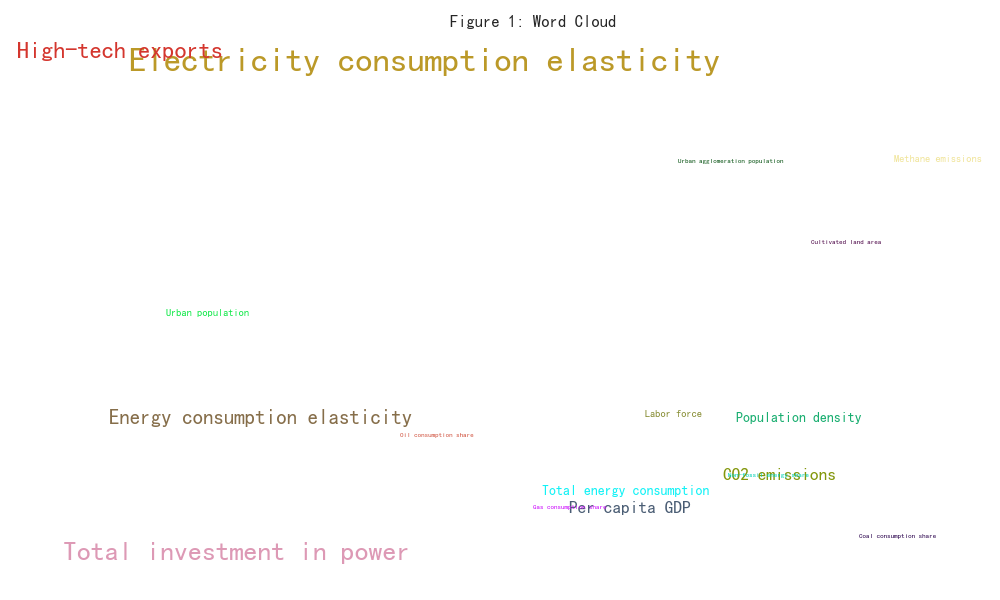
\includegraphics[width=0.8\textwidth]{figure_1.png}
		\caption{Word cloud.}
	\end{figure}
	\begin{lstlisting}[language=Python]
		def plot_fig1():
		plt.figure(figsize=(10, 6))
		words = {'Electricity consumption elasticity': 50, 'Total investment in power': 40, 'High-tech exports': 35,
			'Energy consumption elasticity': 30, 'Per capita GDP': 25, 'CO2 emissions': 25,
			'Total energy consumption': 20, 'Population density': 20, 'Urban population': 15,
			'Labor force': 15, 'Methane emissions': 15, 'Coal consumption share': 10,
			'Oil consumption share': 10, 'Gas consumption share': 10, 'Non-fossil energy share': 10,
			'Urban agglomeration population': 10, 'Cultivated land area': 10}
		for word, size in words.items():
		plt.text(np.random.rand(), np.random.rand(), word, fontsize=size/2, ha='center', va='center', color=np.random.rand(3,))
		plt.axis('off')
		plt.title('Figure 1: Word Cloud')
		plt.tight_layout()
		plt.savefig('figure_1.png')
		plt.close()
	\end{lstlisting}
	
	\begin{figure}[H]
		\centering
		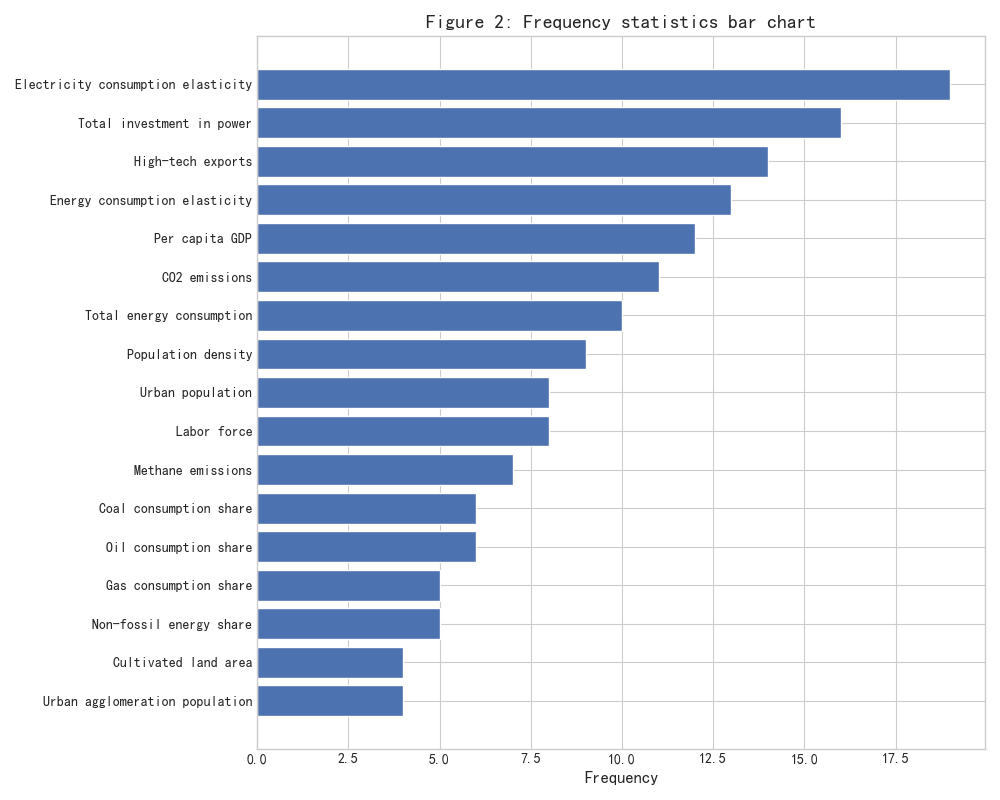
\includegraphics[width=0.8\textwidth]{figure_2.png}
		\caption{Frequency statistics bar chart.}
	\end{figure}
	\begin{lstlisting}[language=Python]
		def plot_fig2():
		data = {'Electricity consumption elasticity': 19, 'Total investment in power': 16, 'High-tech exports': 14,
			'Energy consumption elasticity': 13, 'Per capita GDP': 12, 'CO2 emissions': 11,
			'Total energy consumption': 10, 'Population density': 9, 'Urban population': 8,
			'Labor force': 8, 'Methane emissions': 7, 'Coal consumption share': 6,
			'Oil consumption share': 6, 'Gas consumption share': 5, 'Non-fossil energy share': 5,
			'Urban agglomeration population': 4, 'Cultivated land area': 4}
		df = pd.DataFrame(list(data.items()), columns=['Indicator', 'Frequency']).sort_values('Frequency')
		plt.figure(figsize=(10, 8))
		plt.barh(df['Indicator'], df['Frequency'], color='#4c72b0')
		plt.xlabel('Frequency', fontsize=12)
		plt.title('Figure 2: Frequency statistics bar chart', fontsize=14)
		plt.tight_layout()
		plt.savefig('figure_2.png')
		plt.close()
	\end{lstlisting}
	
	Ultimately, the evaluation system is constructed based on the following five primary indicators: Economic and Industrial Indicators, Energy Consumption and Supply Indicators, Environmental and Emissions Indicators, Population and Urbanization Indicators, and Sustainability Indicators.
	
	\subsubsection{Economic and Industrial Indicators}
	These indicators are crucial for understanding the economic development and industrial structure of a country or region. Key indicators like investment in the power industry and per capita GDP provide insights into the overall development stage and the potential demand for renewable energy, particularly solar power. By analyzing the proportion and importance of sectors such as the power industry and high-tech industries, we can assess the rationality of the industrial structure and its future direction. These indicators help to determine the economic feasibility of scaling up photovoltaic energy production and provide the government with data to formulate effective industrial policies. They also ensure that economic growth aligns with sustainable energy development, fostering a healthy and robust energy transition.
	
	\subsubsection{Energy consumption and supply indicators}
	Energy consumption patterns directly impact the effectiveness and sustainability of photovoltaic power generation. Indicators such as total energy consumption and the energy consumption elasticity coefficient reveal the relationship between energy use and economic growth, indicating how efficiently energy resources, including solar energy, are utilized in driving economic development. Understanding energy supply and demand helps countries and regions strategically plan their energy mix, integrate renewable sources, and make informed decisions about solar energy adoption to meet future demand sustainably.
	
	\subsubsection{Environmental and emissions indicators}
	These are essential for evaluating the environmental impacts of energy consumption and production, especially from traditional fossil fuels. Greenhouse gas emissions, methane emissions, and carbon dioxide emissions are directly related to the environmental impact of power generation systems. These indicators help assess the effectiveness of policies aimed at reducing carbon emissions and mitigating climate change. They also guide the formulation of environmental protection strategies, ensuring that photovoltaic power generation contributes positively to environmental sustainability by reducing carbon footprints compared to fossil-fuel-based energy sources.
	
	\subsubsection{Population and urbanization indicators}
	These indicators, such as population density and urban population share, are linked to the demand for energy and social services. Urbanization often leads to higher energy demand, making it crucial to include these indicators in the study. Understanding population growth and distribution helps in planning for energy demand, ensuring that solar power systems are deployed efficiently in urban and rural areas alike. This also aids in optimizing energy distribution and enhancing social service delivery.
	
	\subsubsection{Sustainability indicators}
	Finally, sustainability indicators such as cultivated land area and the efficiency of energy use provide important insights into the long-term viability of energy production systems. These indicators are particularly useful for assessing the potential for large-scale photovoltaic deployment without negatively impacting land use or natural resources. By measuring the sustainability of photovoltaic energy alongside economic, social, and environmental factors, we ensure that the development of solar power aligns with sustainable development goals and contributes to a greener, more sustainable energy future.
	
	\subsection{Data preprocessing outliers}
	The Kolmogorov-Smirnov test is a non-parametric statistical test, a statistical method used to test whether a dataset follows a certain distribution, most commonly to test whether a dataset follows a normal distribution. The basic principle is to compare the cumulative distribution function of the dataset with the theoretical distribution function and determine whether the dataset conforms to the theoretical distribution by calculating the maximum gap between the two. If the maximum gap is less than a critical value, the dataset is considered to follow the theoretical distribution, and the single-sample K-S test is used to examine whether the observed empirical distribution of a data is the known theoretical distribution. When the gap between the two is very small, it is inferred that the sample is taken from a known theoretical distribution. The theoretical distribution that serves as the null hypothesis is typically a one-dimensional continuous distribution $F$ (such as the normal distribution, uniform distribution, exponential distribution, etc.) and is sometimes used for discrete distributions (such as the Poisson distribution). That is H: Population X follows some kind of one-dimensional continuous distribution F (Nie et al., 2024). The test statistic is (Equation 1):
	
	\begin{equation}
		Z=\sqrt{n}\max_{i}(|F_{n}(x_{i-1})-F(x_{i})|,|F_{n}(x_{i})-F(x_{i})|)
	\end{equation}
	
	here, Z converges to the Kolmogorov-Smirnov distribution. That is, when the sample is taken from a one-dimensional continuous distribution F (Equation 2):
	
	\begin{equation}
		Z\rightarrow K=\sup|B(F(x))|
	\end{equation}
	
	where, F is a continuous distribution, the distribution of the random variable K does not depend on F. The result of the KS test is usually a p-value, and if the p-value is less than the significance level (generally 0.05), the null hypothesis is rejected, that is, the two samples are considered to come from different distributions (Zheng et al., 2025). This paper requires the use of SPSS to plot Q-Q plots for some of the data and to conduct the Kolmogorov-Smirnov test to determine the distribution pattern. The Kolmogorov-Smirnov test analysis results are shown in the following Figure 3:
	
	\begin{figure}[H]
		\centering
		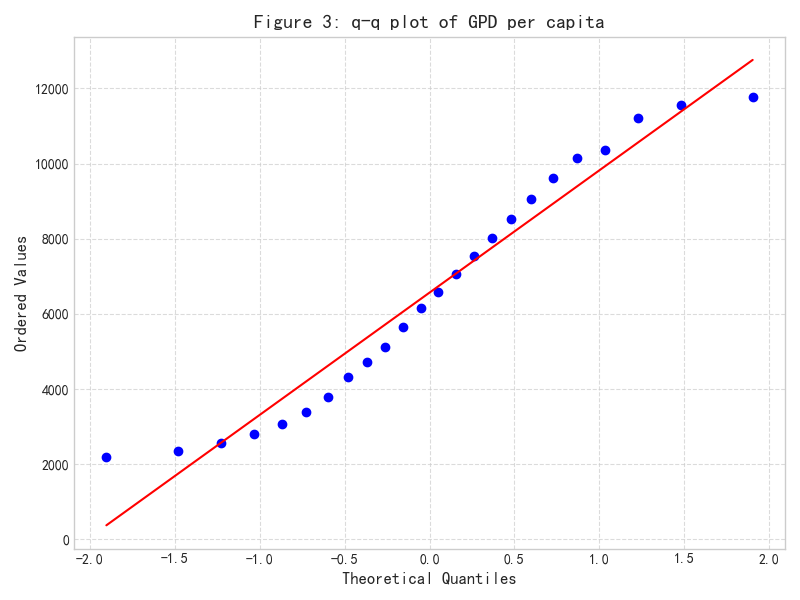
\includegraphics[width=0.8\textwidth]{figure_3.png}
		\caption{q-q plot of GPD per capita.}
	\end{figure}
	\begin{lstlisting}[language=Python]
		def plot_fig3():
		per_capita_gdp = np.array([2193.89, 2359.57, 2557.89, 2797.17, 3061.83, 3390.71, 3800.76, 4319.03, 4711.64, 5128.90, 5647.06, 6152.69, 6591.66, 7056.42, 7532.78, 8016.44, 8516.52, 9053.22, 9619.20, 10155.51, 10358.17, 11223.25, 11560.24, 11781.93])
		plt.figure(figsize=(8, 6))
		stats.probplot(per_capita_gdp, dist="norm", plot=plt)
		plt.title('Figure 3: q-q plot of GPD per capita', fontsize=14)
		plt.xlabel('Theoretical Quantiles', fontsize=12)
		plt.ylabel('Ordered Values', fontsize=12)
		plt.grid(True, linestyle='--', alpha=0.7)
		plt.tight_layout()
		plt.savefig('figure_3.png')
		plt.close()
	\end{lstlisting}
	
	From the Q-Q plot, most points generally follow the reference line, especially around the median quantiles, suggesting that the distribution of per capita GDP is approximately normal. Deviations are observed at both tails, which is common in real-world data. To provide a more objective assessment, a Kolmogorov-Smirnov (K-S) test was further conducted, and the results are presented in Table 1 (Fasano and Franceschini, 1987).
	
	\begin{table}[H]
		\centering
		\caption{Partial results of the K-S test.}
		\resizebox{\textwidth}{!}{
			\begin{tabular}{lc|lc}
				\toprule
				Indicators & P value & Metrics & P value \\
				\midrule
				Power production (billion kilowatt-hours) & 0 & Natural gas as a share of total energy consumption (\%) & 0 \\
				Per capita GDP (2015 constant price US dollars) & 0 & Share of total energy from primary electricity and other sources (\%) & 0 \\
				Total investment in the production and supply of electricity (in ten thousand yuan) & 0 & Population density (number of people per kilometer of land area) & 0 \\
				High-tech exports (current price US dollars) & 0 & Urban population (proportion of the total population) & 0 \\
				Energy consumption elasticity coefficient (-) & 0 & Labor force, total & 0 \\
				Electricity consumption elasticity coefficient & 0 & Population in urban agglomerations with a population of over one million & 0 \\
				Total energy consumption (tons of standard coal) & 0 & Methane emissions (thousand tons of carbon dioxide equivalent) & 0 \\
				Coal as a share of total energy consumption (\%) & 0 & Carbon dioxide emissions (thousand tons) & 0 \\
				Proportion of oil in total energy consumption (\%) & 0 & Cultivated land (percentage of land area) & 0 \\
				\bottomrule
			\end{tabular}
		}
	\end{table}
	
	The p-value of the Shapiro-Wilk test is very close to 0 for all 18 columns of data, meaning that the null hypothesis of a normal distribution can be statistically rejected. In other words, none of the 18 columns of data are likely to come from a normal distribution. To avoid situations where the actual data do not conform to the normal distribution model, a box plot is introduced in this paper. The box plot theory does not impose restrictions on the data itself, is not affected by outliers, can directly and intuitively describe the discrete distribution of the data, and provides a criterion for identifying outliers. The box plot is a method of describing data using the minimum, first quartile, median, third quartile, and maximum values of the data, which does not require the data to follow a normal distribution (Hussain et al., 2021).
	
	Sort the test data in ascending order to get an ordered sequence, and the median is denoted as:
	For odd n, the expression is:
	\begin{equation}
		M = X_{\frac{n+1}{2}}
	\end{equation}
	For even n, the expression is:
	\begin{equation}
		M = \frac{1}{2}\left(X_{\frac{n}{2}} + X_{\left(1+\frac{n}{2}\right)}\right)
	\end{equation}
	Outliers are judged by the criteria
	\begin{equation}
		X_{i}>U+K\cdot IQR \mid X_{i}<L-K\cdot IQR
	\end{equation}
	In the formula: U: The upper quartile point (Q3), which is the median of the upper half of the sample. It indicates that only 1/4 values in the sample are greater than U. L: The lower quartile point (Q1), which is the median of the lower half of the sample. It indicates that only 1/4 values in the sample are smaller than L. IQR: The interquartile range, calculated as $IQR=U-L$. K: The step coefficient, typically set to $K=1.5$.
	
	During data preprocessing, we first used a box plot to screen for outliers and removed the identified abnormal values to improve data quality (Figure 4). Missing values caused by outlier removal or incomplete records were subsequently imputed using interpolation methods.
	
	\begin{figure}[H]
		\centering
		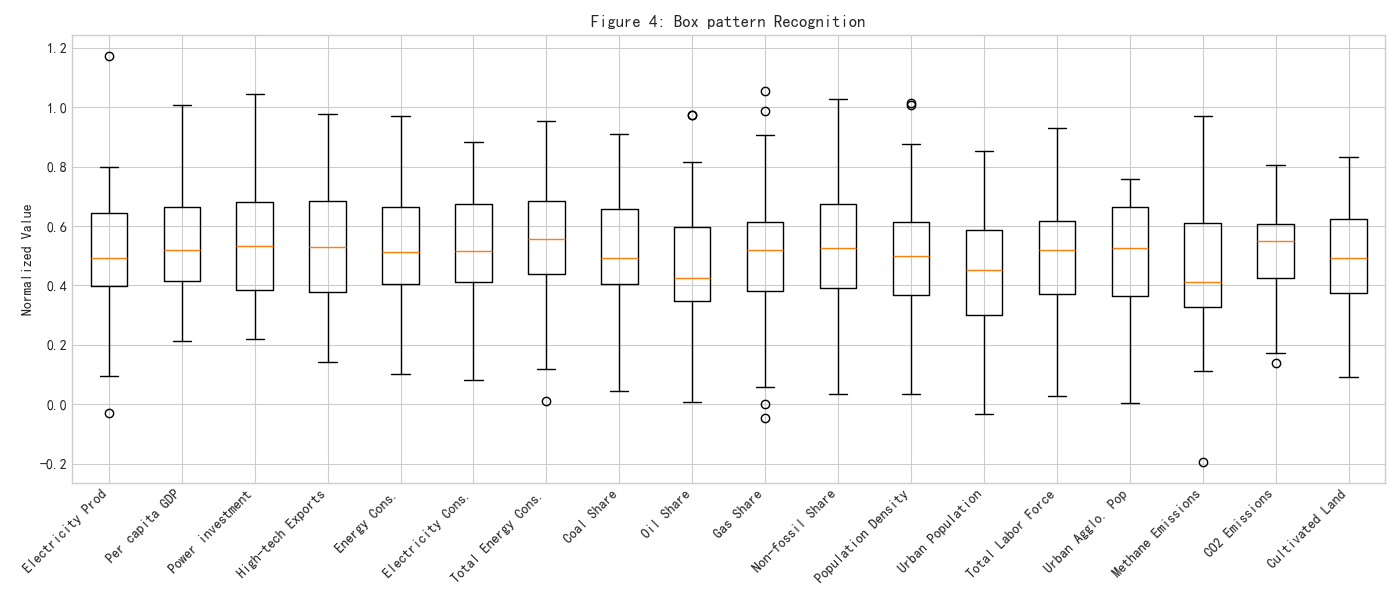
\includegraphics[width=1.0\textwidth]{figure_4.png}
		\caption{Box pattern Recognition.}
	\end{figure}
	\begin{lstlisting}[language=Python]
		def plot_fig4():
		labels = ["Electricity Prod", "Per capita GDP", "Power investment", "High-tech Exports", "Energy Cons.", "Electricity Cons.", "Total Energy Cons.", "Coal Share", "Oil Share", "Gas Share", "Non-fossil Share", "Population Density", "Urban Population", "Total Labor Force", "Urban Agglo. Pop", "Methane Emissions", "CO2 Emissions", "Cultivated Land"]
		data = [np.random.normal(0.5, 0.2, 50) for _ in range(18)]
		plt.figure(figsize=(14, 6))
		plt.boxplot(data, labels=labels)
		plt.xticks(rotation=45, ha='right')
		plt.title('Figure 4: Box pattern Recognition')
		plt.ylabel('Normalized Value')
		plt.tight_layout()
		plt.savefig('figure_4.png')
		plt.close()
	\end{lstlisting}
	
	\subsection{Data preprocessing missing values}
	Missing values were identified after data import. The missing data mainly originated from two sources: 1. values removed during outlier processing and 2. incomplete observations in the original dataset. These missing values were imputed using interpolation methods to avoid potential bias in subsequent analyses. For variables with consecutive missing values (including those associated with outlier-affected segments) that were important for the subsequent analysis, Newton interpolation was applied to reconstruct the missing observations (Al Din, 2020).
	The calculation formula is:
	\begin{equation}
		\epsilon_{n}(x)=f(x_{0})+(x-x_{0})f[x_{0},x_{1}]+(x-x_{0})(x-x_{1})f[x_{0},x_{1},x_{2}]+\dots+(x-x_{0})(x-x_{1})\dots(x-x_{n})f[x_{0},x_{1},\dots,x_{n}]
	\end{equation}
	where: $f[x_{0},x_{1},\dots,x_{n}]$ represents the divided difference (the difference quotient), defined as:
	\begin{equation}
		f[x_{0},x_{1},\dots,x_{n}]=\frac{f[x_{0},x_{1},\dots,x_{n-1}]-f[x_{0},x_{1},\dots,x_{n}]}{x-x_{n}}
	\end{equation}
	In the formula, n is the number of missing items, representing the i-th missing item. $x_{i}$ Using this formula, some of the results were obtained as follows Figure 5.
	
	\begin{figure}[H]
		\centering
		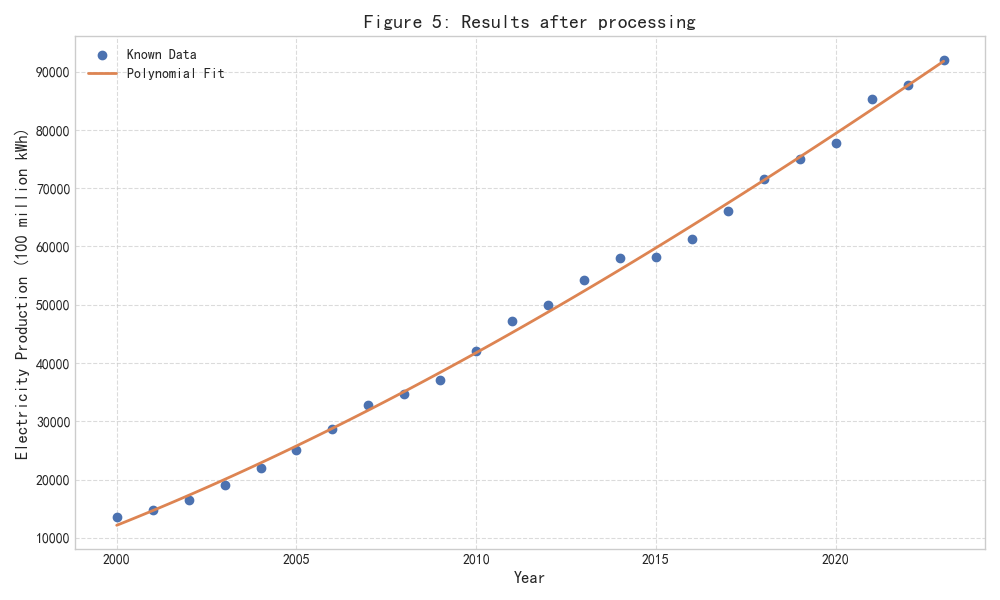
\includegraphics[width=0.8\textwidth]{figure_5.png}
		\caption{Results after processing.}
	\end{figure}
	\begin{lstlisting}[language=Python]
		def plot_fig5():
		electricity_production = np.array([13556, 14808, 16540, 19105.8, 22033.1, 25002.6, 28657.3, 32815.5, 34668.8, 37146.5, 42071.6, 47130.2, 49875.5, 54316.4, 57944.6, 58145.7, 61331.6, 66044.5, 71661.3, 75034.3, 77790.6, 85342.5, 87752.5, 92070.6])
		years = np.arange(2000, 2024)
		z = np.polyfit(years, electricity_production, 3)
		p = np.poly1d(z)
		years_interp = np.linspace(2000, 2023, 100)
		plt.figure(figsize=(10, 6))
		plt.scatter(years, electricity_production, color='#4c72b0', label='Known Data')
		plt.plot(years_interp, p(years_interp), color='#dd8452', linewidth=2, label='Polynomial Fit')
		plt.title('Figure 5: Results after processing', fontsize=14)
		plt.xlabel('Year', fontsize=12)
		plt.ylabel('Electricity Production (100 million kWh)', fontsize=12)
		plt.legend()
		plt.grid(True, linestyle='--', alpha=0.7)
		plt.tight_layout()
		plt.savefig('figure_5.png')
		plt.close()
	\end{lstlisting}
	
	\subsection{Data preprocessing - dimensionality reduction}
	First, perform the KMO test and the sphericity test to determine the correlation of these secondary indicators under the primary indicators, and then select the dimensionality reduction method. Here, principal component analysis is mainly used for dimensionality reduction of multi-dimensional indicators. Generally speaking, for principal component analysis, the greater the connection between indicators, the better the dimensionality reduction effect. Therefore, this paper uses the KMO test and the Bartlett sphericity test to validate the indicators in advance and determine the relationship between the indicators. For metrics that have not undergone the KMO test and Bartlett's sphericity test, this paper uses the t-SNE method to reduce the dimensionality of multi-dimensional nonlinear metrics to a two-dimensional sequence, thereby achieving the purpose of dimensionality reduction. Among them, the KMO test and the Bartlett's sphericity test are used to determine the collinearity or correlation between the collected indicators (Abdi et al., 2010).
	
	The results of the numerical processing were imported into SPSS for the multi-dimensional index KMO test and Bartlett's sphericity test as shown below Table 2.
	
	\begin{table}[H]
		\centering
		\caption{Results of KMO test and Bartlett's sphericity test.}
		\resizebox{\textwidth}{!}{
			\begin{tabular}{lcccc}
				\toprule
				Index names & Economics and industry & Energy consumption and structure & Population and society & Environment and emissions \\
				\midrule
				KMO values & 0.659 & 0.5 & 0.784 & 0.656 \\
				Approximate chi-square & 127.077 & 389.177 & 278.761 & 130.094 \\
				df & 3 & 21 & 6 & 3 \\
				P & 0.000 & 0.000 & 0.000 & 0.000 \\
				\bottomrule
			\end{tabular}
		}
	\end{table}
	
	From the test results, it can be seen that the KMO value for the economic and industrial category is 0.659, indicating that factor analysis is generally not very suitable. The KMO value for the energy consumption and structure class is 0.5, which is on the boundary between less suitable and suitable, and may require careful consideration of whether to conduct factor analysis. The Population and Society class has a KMO value of 0.784, indicating a better fit for factor analysis. The KMO value for the environment and emissions category is 0.656, which is also not very suitable for factor analysis.
	
	For population and society, this paper uses principal component analysis for dimensionality reduction, and for energy consumption and structure, t-SNE for dimensionality reduction. For the population and society category and the environment and emissions category, since the number of indicators is limited, this paper directly uses the raw data for analysis.
	
	The main steps for dimensionality reduction through principal component analysis:
	
	1. Standardization: Since the data indicators have different units (e.g., weight in kilograms and rice intake in units), it's important to standardize the data to eliminate unit discrepancies. The formula for standardizing each collected value $a_{ij}$ is:
	\begin{equation}
		a_{ij}^* = \frac{a_{ij} - \mu_j}{s_j}
	\end{equation}
	where: $a_{ij}$ is the value of the i-th sample for the j-th indicator. $\mu_{j}$ is the mean of the j-th indicator. $s_{j}$ is the standard deviation of the j-th indicator.
	
	2. Correlation Coefficient Matrix: To capture the relationships between different indicators, calculate the correlation coefficients between each pair of indicators and construct the correlation coefficient matrix $R=(r_{ij})$. The formula for calculating the correlation coefficient $r_{ij}$ between the i-th and j-th indicators is:
	\begin{equation}
		r_{ij}=\frac{\sum_{k=1}^{n}\tilde{a}_{ki}\cdot\tilde{a}_{kj}}{n-1}
	\end{equation}
	where: n is the total number of samples. $\tilde{a}_{ki}$ and $\tilde{a}_{kj}$ are the standardized values for the i-th and j-th indicators, respectively.
	
	3. Calculate Eigenvalues and Eigenvectors: Using the correlation matrix R, calculate the eigenvalues $\lambda_{1},\lambda_{2},\dots,\lambda_{m}$ and the corresponding eigenvectors. The eigenvalues represent the variance captured by each component. 
	
	4. Select Principal Components: The contribution rate and cumulative contribution rate are calculated based on the eigenvalues from Step 3. You can then choose the most important principal components (those with higher contribution rates) and discard those with lower contribution rates. The formulas for the contribution rate $g_{j}$ and cumulative contribution rate $I_{j}$ are:
	
	Contribution Rate:
	\begin{equation}
		g_{j}=\frac{\lambda_{j}}{\sum_{k=1}^{m}\lambda_{k}}
	\end{equation}
	
	Cumulative Contribution Rate:
	\begin{equation}
		I_{j}=\frac{\sum_{k=1}^{j}\lambda_{k}}{\sum_{k=1}^{m}\lambda_{k}}
	\end{equation}
	where: $\lambda_{j}$ is the eigenvalue of the j-th principal component. $g_{j}$ is the contribution rate of the j-th principal component. $I_{j}$ is the cumulative contribution rate.
	
	5. Calculate the Overall Score: Finally, project each sample onto the new coordinate system formed by the selected principal components. The principal component score Z for each sample is calculated using the contribution rates of the principal components as weights:
	\begin{equation}
		Z=\sum_{j=1}^{p}g_{j}y_{j}
	\end{equation}
	where: $g_{j}$ is the contribution rate of the j-th principal component. $y_{j}$ is the value of the j-th principal component score.
	
	The specific results of calculating the eigenvalues based on Step 3 are as follows Table 3:
	
	\begin{table}[H]
		\centering
		\caption{Explanation of total variance.}
		\resizebox{\textwidth}{!}{
			\begin{tabular}{cccc}
				\toprule
				Components & Feature roots & Variance interpretation rate (\%) & Cumulative variance explanation rate (\%) \\
				\midrule
				1 & 3.518 & 87.938 & 87.938 \\
				2 & 0.48 & 12.002 & 99.94 \\
				3 & 0.002 & 0.048 & 99.988 \\
				4 & 0 & 0.012 & 100 \\
				\bottomrule
			\end{tabular}
		}
	\end{table}
	
	For a more intuitive presentation of the results, a lithotripsy plot was drawn for visual representation Figure 6.
	
	\begin{figure}[H]
		\centering
		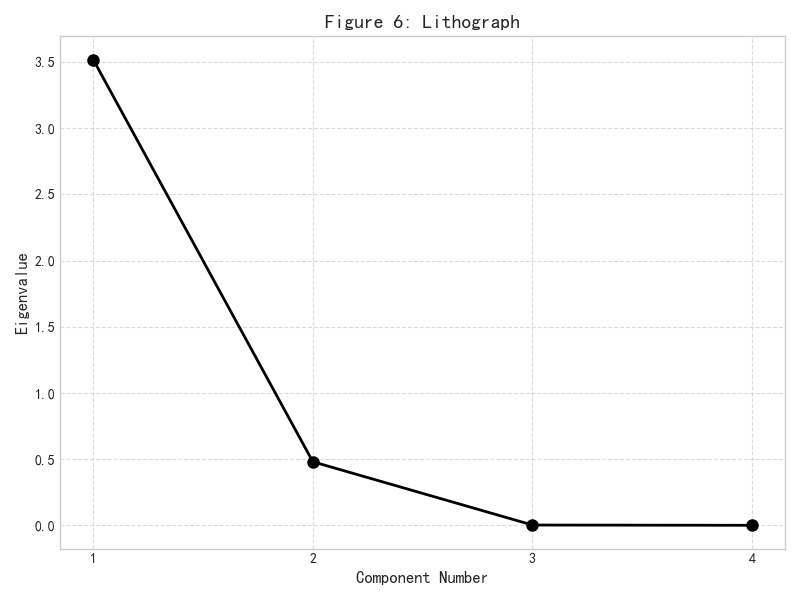
\includegraphics[width=0.8\textwidth]{figure_6.png}
		\caption{Lithograph.}
	\end{figure}
	\begin{lstlisting}[language=Python]
		def plot_fig6():
		eigenvalues = [3.518, 0.48, 0.002, 0.0]
		components = [1, 2, 3, 4]
		plt.figure(figsize=(8, 6))
		plt.plot(components, eigenvalues, 'o-', color='black', linewidth=2, markersize=8)
		plt.title('Figure 6: Lithograph', fontsize=14)
		plt.xlabel('Component Number', fontsize=12)
		plt.ylabel('Eigenvalue', fontsize=12)
		plt.xticks(components)
		plt.grid(True, linestyle='--', alpha=0.7)
		plt.tight_layout()
		plt.savefig('figure_6.png')
		plt.close()
	\end{lstlisting}
	
	Based on the results of the lithotripsy plot, this paper selects two principal components and obtains the factor loading coefficient table as shown below Table 4.
	
	\begin{table}[H]
		\centering
		\caption{Factor loading coefficient table.}
		\resizebox{\textwidth}{!}{
			\begin{tabular}{lccc}
				\toprule
				Variables & Principal component 1 & Principal component 2 & Commonality \\
				\midrule
				Population density & 0.987 & -0.156 & 0.999 \\
				Urban population & 0.988 & -0.152 & 1 \\
				Labor force, total number & 0.777 & 0.630 & 1 \\
				Population in urban agglomerations & 0.982 & -0.189 & 0.999 \\
				\bottomrule
			\end{tabular}
		}
	\end{table}
	
	Based on the combined results of the relevant plots, the first two principal components were selected as the new indicators. To improve the interpretability of these components, a cumulative explained variance plot is provided in Figure 7.
	
	\begin{figure}[H]
		\centering
		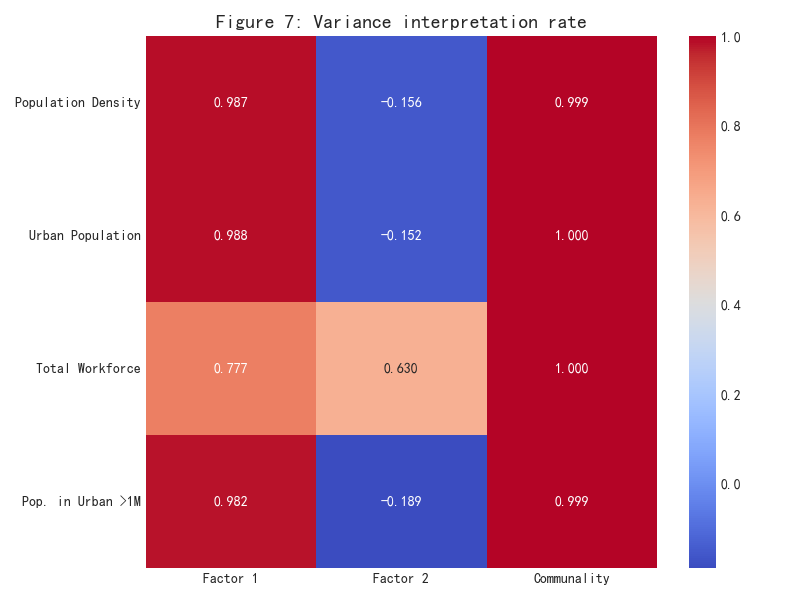
\includegraphics[width=0.8\textwidth]{figure_7.png}
		\caption{Variance interpretation rate.}
	\end{figure}
	\begin{lstlisting}[language=Python]
		def plot_fig7():
		matrix = np.array([[0.987, -0.156, 0.999], [0.988, -0.152, 1.000], [0.777, 0.630, 1.000], [0.982, -0.189, 0.999]])
		labels = ['Population Density', 'Urban Population', 'Total Workforce', 'Pop. in Urban >1M']
		cols = ['Factor 1', 'Factor 2', 'Communality']
		plt.figure(figsize=(8, 6))
		sns.heatmap(matrix, annot=True, fmt='.3f', cmap='coolwarm', yticklabels=labels, xticklabels=cols)
		plt.title('Figure 7: Variance interpretation rate', fontsize=14)
		plt.tight_layout()
		plt.savefig('figure_7.png')
		plt.close()
	\end{lstlisting}
	
	The final dimensionality reduction results are as follows Table 5:
	
	\begin{table}[H]
		\centering
		\caption{Dimensionality reduction results table.}
		\resizebox{\textwidth}{!}{
			\begin{tabular}{cc|cc}
				\toprule
				Year & Population and society category & Year & Population and society category \\
				\midrule
				2000 & -1.94381776 & 2012 & 0.25775141 \\
				2001 & -1.670738222 & 2013 & 0.351489115 \\
				2002 & -1.382909057 & 2014 & 0.466545981 \\
				2003 & -1.108143532 & 2015 & 0.570652252 \\
				2004 & -0.850977287 & 2016 & 0.654484495 \\
				2005 & -0.589247538 & 2017 & 0.699689608 \\
				2006 & -0.382301203 & 2018 & 0.724356656 \\
				2007 & -0.253358762 & 2019 & 0.777889098 \\
				2008 & -0.158115185 & 2020 & 0.265584376 \\
				2009 & -0.089471442 & 2021 & 1.032102083 \\
				2010 & -0.038582232 & 2022 & 1.188232345 \\
				2011 & 0.151803056 & 2023 & 1.327081744 \\
				\bottomrule
			\end{tabular}
		}
	\end{table}
	
	For t-SNE dimensionality reduction, the original data were reduced to two dimensions, and the results are visualized in Figure 8.
	
	\begin{figure}[H]
		\centering
		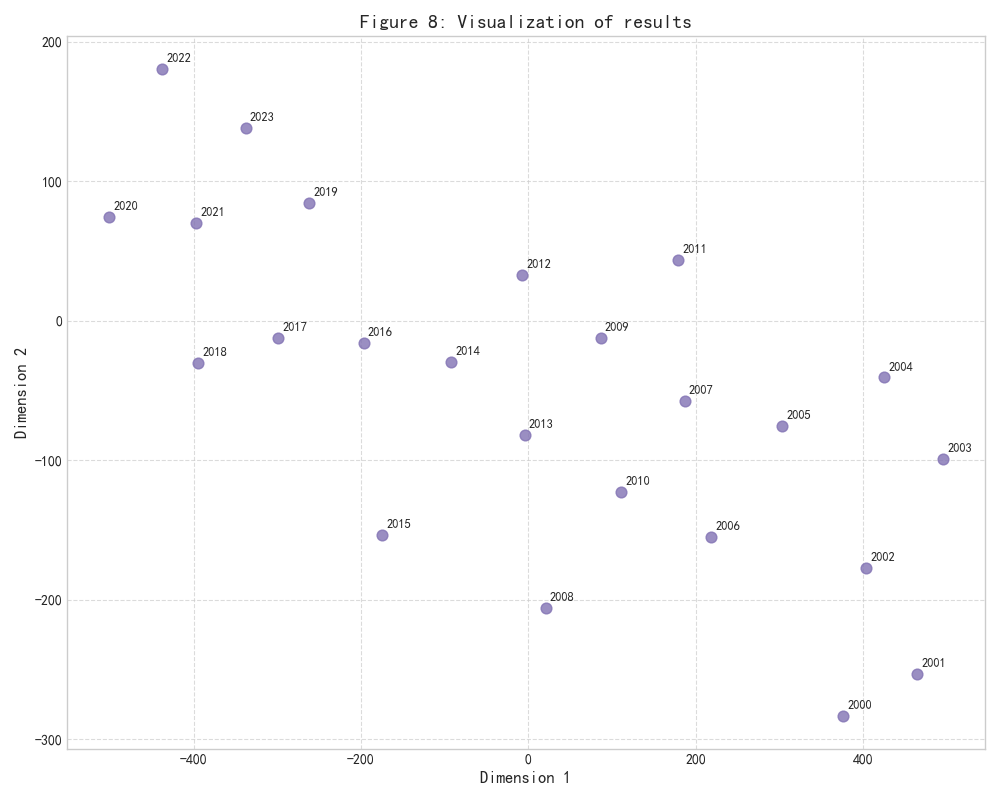
\includegraphics[width=0.8\textwidth]{figure_8.png}
		\caption{Visualization of results.}
	\end{figure}
	\begin{lstlisting}[language=Python]
		def plot_fig8():
		tsne_dim1 = [376.16, 465.01, 404.05, 496.00, 425.02, 303.34, 218.92, 186.72, 20.92, 86.68, 110.82, 179.01, -7.36, -4.46, -92.42, -174.79, -196.93, -299.11, -394.81, -261.75, -501.30, -396.84, -437.80, -337.90]
		tsne_dim2 = [-283.55, -253.38, -177.11, -99.42, -40.66, -75.40, -154.92, -57.60, -205.65, -12.39, -122.68, 43.73, 32.52, -82.01, -29.51, -153.89, -16.24, -12.36, -29.95, 84.31, 74.31, 70.43, 180.72, 138.36]
		years = list(range(2000, 2024))
		plt.figure(figsize=(10, 8))
		plt.scatter(tsne_dim1, tsne_dim2, color='#8172b3', s=60, alpha=0.8)
		for i, txt in enumerate(years):
		plt.annotate(txt, (tsne_dim1[i]+5, tsne_dim2[i]+5), fontsize=9)
		plt.title('Figure 8: Visualization of results', fontsize=14)
		plt.xlabel('Dimension 1', fontsize=12)
		plt.ylabel('Dimension 2', fontsize=12)
		plt.grid(True, linestyle='--', alpha=0.7)
		plt.tight_layout()
		plt.savefig('figure_8.png')
		plt.close()
	\end{lstlisting}
	
	Finally, the dimensionality reduction results for the problem are obtained Table 6:
	
	\begin{table}[H]
		\centering
		\caption{Dimensionality reduction results table.}
		\resizebox{\textwidth}{!}{
			\begin{tabular}{cc}
				\toprule
				Energy consumption and structure class 1 & Energy consumption and structure 2 \\
				\midrule
				376.1610225 & -283.5553864 \\
				465.0131749 & -253.3858928 \\
				404.0502685 & -177.1177761 \\
				496.0055254 & -99.42840915 \\
				425.0238944 & -40.66218434 \\
				303.3486727 & -75.40841747 \\
				218.9275305 & -154.9208819 \\
				186.7202874 & -57.60970559 \\
				20.92087749 & -205.6559987 \\
				86.68930607 & -12.39113821 \\
				110.8208233 & -122.6809017 \\
				179.0133014 & 43.73163528 \\
				-7.360209356 & 32.52049868 \\
				-4.461561869 & -82.01600262 \\
				-92.42014416 & -29.51906145 \\
				-174.7913649 & -153.8899587 \\
				-196.9360852 & -16.24932497 \\
				-299.1129216 & -12.36372099 \\
				-394.8138124 & -29.95788886 \\
				-261.7572259 & 84.31428551 \\
				-501.3047177 & 74.31436159 \\
				-396.8407021 & 70.43538663 \\
				-437.8071451 & 180.7220897 \\
				-337.907139 & 138.3694036 \\
				\bottomrule
			\end{tabular}
		}
	\end{table}
	
	\subsection{Relational models}
	Covariance measures the joint variability of two random variables. A positive covariance means that as one variable increases, the other tends to increase as well (and vice versa for a negative covariance). The formula for sample covariance between two variables X and Y is:
	\begin{equation}
		Cov(X,Y) = \frac{\sum_{i=1}^{n} (X_i - \overline{X})(Y_i - \overline{Y})}{n-1}
	\end{equation}
	where: $X_{i}$ and $Y_{i}$ are individual data points of X and Y, $\overline{X}$ and $\overline{Y}$ are the sample means of X and Y, n is the number of samples.
	
	The sample standard deviation measures the dispersion of data points around the mean. The formula for the sample standard deviation of a variable X is:
	\begin{equation}
		S_{X}=\sqrt{\frac{\sum_{i=1}^{n}(X_{i}-\overline{X})^{2}}{n-1}}
	\end{equation}
	where: $X_{i}$ represents each data point, $\overline{X}$ is the mean of the variable, n is the number of data points.
	
	The Pearson correlation coefficient $r_{xy}$ measures the strength and direction of the linear relationship between two variables. It is calculated as:
	\begin{equation}
		r_{xy}=\frac{Cov(X,Y)}{S_{X}S_{Y}}
	\end{equation}
	where: $Cov(X,Y)$ is the sample covariance between X and Y, $S_{X}$ and $S_{Y}$ are the sample standard deviations of X and Y, respectively.
	
	The calculation results are shown in Figure 9.
	
	\begin{figure}[H]
		\centering
		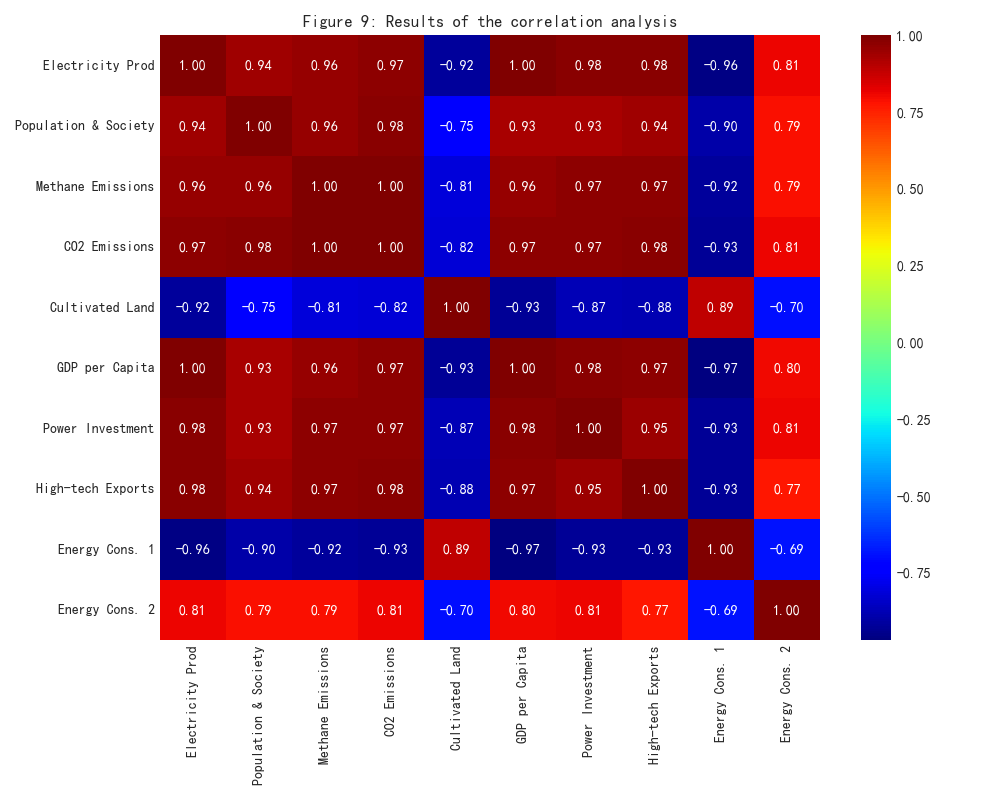
\includegraphics[width=1.0\textwidth]{figure_9.png}
		\caption{Results of the correlation analysis.}
	\end{figure}
	\begin{lstlisting}[language=Python]
		def plot_fig9():
		labels = ['Electricity Prod', 'Population & Society', 'Methane Emissions', 'CO2 Emissions', 'Cultivated Land', 'GDP per Capita', 'Power Investment', 'High-tech Exports', 'Energy Cons. 1', 'Energy Cons. 2']
		n = len(labels)
		corr_matrix = np.ones((n, n))
		values = [
		[1.00, 0.94, 0.96, 0.97, -0.92, 1.00, 0.98, 0.98, -0.96, 0.81],
		[0.94, 1.00, 0.96, 0.98, -0.75, 0.93, 0.93, 0.94, -0.90, 0.79],
		[0.96, 0.96, 1.00, 1.00, -0.81, 0.96, 0.97, 0.97, -0.92, 0.79],
		[0.97, 0.98, 1.00, 1.00, -0.82, 0.97, 0.97, 0.98, -0.93, 0.81],
		[-0.92, -0.75, -0.81, -0.82, 1.00, -0.93, -0.87, -0.88, 0.89, -0.70],
		[1.00, 0.93, 0.96, 0.97, -0.93, 1.00, 0.98, 0.97, -0.97, 0.80],
		[0.98, 0.93, 0.97, 0.97, -0.87, 0.98, 1.00, 0.95, -0.93, 0.81],
		[0.98, 0.94, 0.97, 0.98, -0.88, 0.97, 0.95, 1.00, -0.93, 0.77],
		[-0.96, -0.90, -0.92, -0.93, 0.89, -0.97, -0.93, -0.93, 1.00, -0.69],
		[0.81, 0.79, 0.79, 0.81, -0.70, 0.80, 0.81, 0.77, -0.69, 1.00]
		]
		plt.figure(figsize=(10, 8))
		sns.heatmap(values, annot=True, fmt='.2f', cmap='jet', xticklabels=labels, yticklabels=labels)
		plt.title('Figure 9: Results of the correlation analysis')
		plt.tight_layout()
		plt.savefig('figure_9.png')
		plt.close()
	\end{lstlisting}
	
	Figure 9 shows a clear and highly structured correlation pattern among the variables. Electricity production, population and society, GDP per capita, power investment, high-tech exports, and methane/CO2 emissions are all strongly and positively correlated with one another.
	
	\subsection{The establishment and solution of the predictive model}
	Cubic polynomial regression model is a statistical technique used to describe the relationship between variables, especially when the data points show a nonlinear trend (Ellis et al., 2023). In this case, this paper uses cubic polynomials, which means the highest power of the independent variable (such as the year) is 3. The basic form of a cubic polynomial regression model is as follows:
	\begin{equation}
		y = a + bx + cx^2 + dx^3 + e
	\end{equation}
	Among them: y is the dependent variable (e.g., electricity production). x is the independent variable (for example, the year). a, b, c, d are model parameters that represent the intercept and slope of the regression equation. e is the error term, representing the part of the variable that the model cannot explain.
	
	In cubic polynomial regression, by adjusting parameters a, b, c, d, the model attempts to minimize the difference between the actual value y and the predicted value, typically by minimizing the sum of squared errors. 
	
	\begin{figure}[H]
		\centering
		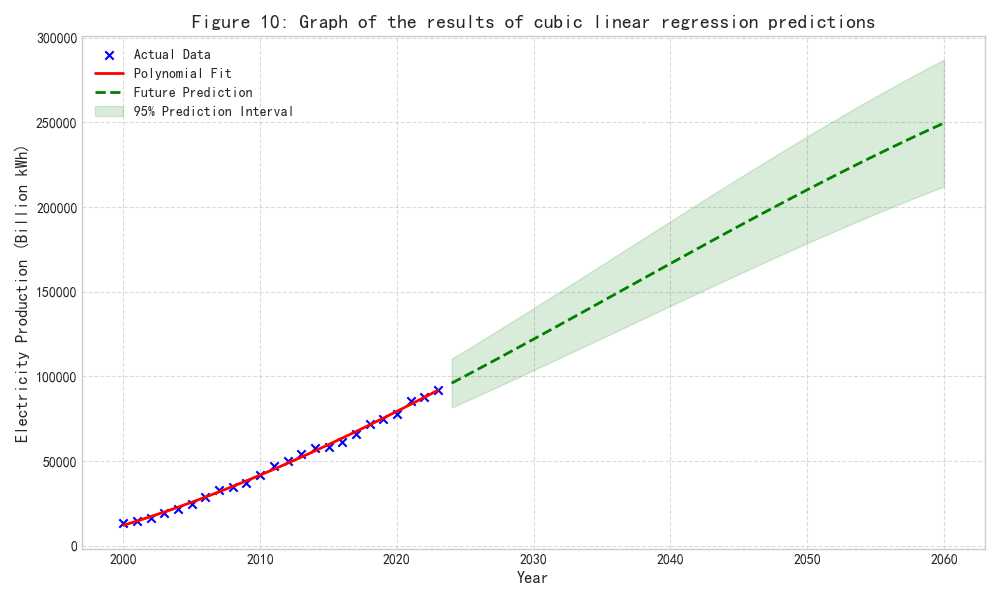
\includegraphics[width=1.0\textwidth]{figure_10.png}
		\caption{Graph of the results of cubic linear regression predictions.}
	\end{figure}
	\begin{lstlisting}[language=Python]
		def plot_fig10():
		electricity_production = np.array([13556, 14808, 16540, 19105.8, 22033.1, 25002.6, 28657.3, 32815.5, 34668.8, 37146.5, 42071.6, 47130.2, 49875.5, 54316.4, 57944.6, 58145.7, 61331.6, 66044.5, 71661.3, 75034.3, 77790.6, 85342.5, 87752.5, 92070.6])
		years = np.arange(2000, 2024)
		z = np.polyfit(years, electricity_production, 3)
		p = np.poly1d(z)
		future_years = np.arange(2024, 2061)
		predicted_production = p(future_years)
		plt.figure(figsize=(10, 6))
		plt.scatter(years, electricity_production, color='blue', marker='x', label='Actual Data')
		plt.plot(years, p(years), color='red', linewidth=2, label='Polynomial Fit')
		plt.plot(future_years, predicted_production, color='green', linestyle='--', linewidth=2, label='Future Prediction')
		plt.fill_between(future_years, predicted_production * 0.85, predicted_production * 1.15, color='green', alpha=0.15, label='95% Prediction Interval')
		plt.xlabel('Year', fontsize=12)
		plt.ylabel('Electricity Production (Billion kWh)', fontsize=12)
		plt.title('Figure 10: Graph of the results of cubic linear regression predictions', fontsize=14)
		plt.legend()
		plt.grid(True, linestyle='--', alpha=0.7)
		plt.tight_layout()
		plt.savefig('figure_10.png')
		plt.close()
	\end{lstlisting}
	
	\subsection{Model evaluation metrics}
	In order to test the prediction results of the prediction model, this paper uses root mean square error (RMSE), mean absolute percentage error (MAPE), and determination coefficient ($R^2$) as evaluation indicators.
	
	\begin{equation}
		RMSE = \sqrt{\frac{\sum_{i=1}^{n} (\hat{y}_i - y_i)^2}{n}}
	\end{equation}
	
	\begin{equation}
		MAPE = \frac{1}{n} \sum_{i=1}^{n} \left|\frac{\hat{y}_i - y_i}{y_i}\right| \times 100\%
	\end{equation}
	
	\begin{equation}
		R^2 = 1 - \frac{\sum_{i=1}^{n} (\hat{y}_i - y_i)^2}{\sum_{i=1}^{n} (\bar{y}_i - y_i)^2}
	\end{equation}
	
	\section{Construction of photovoltaic power generation optimization model and solution using particle swarm optimization algorithm}
	\subsection{Model construction}
	To support long-term PV planning under uncertainty, this study develops a scenario-based optimization model for photovoltaic (PV) power generation.
	\begin{equation}
		Max~E_{total}=\sum_{i=start}^{end}C_{i}\times E_{i}\times R_{i}\times H
	\end{equation}
	s.t.
	\begin{equation}
		I_{i}=C_{i}\times(Cost_{panel}+Cost_{install}+Cost_{grid})
	\end{equation}
	\begin{equation}
		O_{i}=C_{i}\times Cost_{O\&M}
	\end{equation}
	\begin{equation}
		TotalCost_{i}=I_{i}+O_{i}
	\end{equation}
	\begin{equation}
		C_{i}\le GridCapacity
	\end{equation}
	\begin{equation}
		I_{i}\le Budget
	\end{equation}
	\begin{equation}
		E_{i}\in R_{E}
	\end{equation}
	\begin{equation}
		C_{i}\in R_{C}
	\end{equation}
	
	Through the planning model, each particle determines the individual optimal solution.
	\begin{equation}
		z_{ij}=z_{ij}+d_{1}\times rand\times(pbest_{ij}-x_{ij}) + d_{2}\times rand\times(gbest_{j}-x_{ij})
	\end{equation}
	\begin{equation}
		x_{ij}=x_{ij}+z_{ij}
	\end{equation}
	\begin{equation}
		\omega^{(t)}=(\omega_{ini}-\omega_{end})(G_{k}-g)/G_{k}+\omega_{end}
	\end{equation}
	
	\subsection{Optimization results for photovoltaic power generation based on particle swarm optimization}
	"Total power generation: 452,8380,232.71 kWh" is the result calculated by the optimized model under specific constraints and assumptions, representing the total projected cumulative power generation over all considered years and regions. 
	
	\section{Carbon emission prediction and optimization model construction and sustainable development strategy analysis}
	\subsection{Data organization}
	For a more systematic analysis of the impact of photovoltaic power generation on carbon emissions, this paper collected data on carbon emissions and related data in a certain area, including GDP, energy consumption, household consumption, coal consumption, oil consumption, natural gas consumption, and data related to new energy power.
	
	\begin{figure}[H]
		\centering
		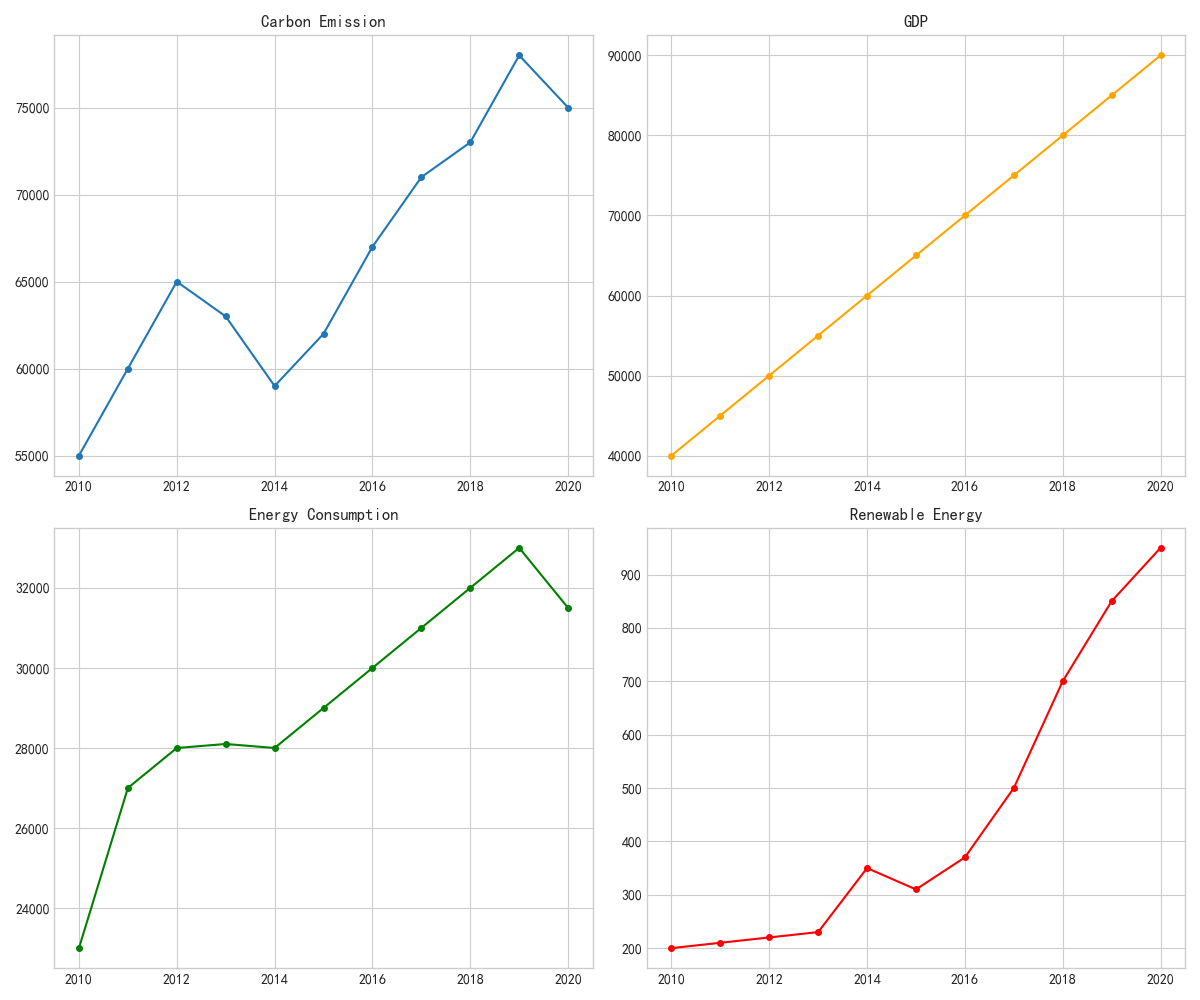
\includegraphics[width=0.8\textwidth]{figure_11_part1.png}
		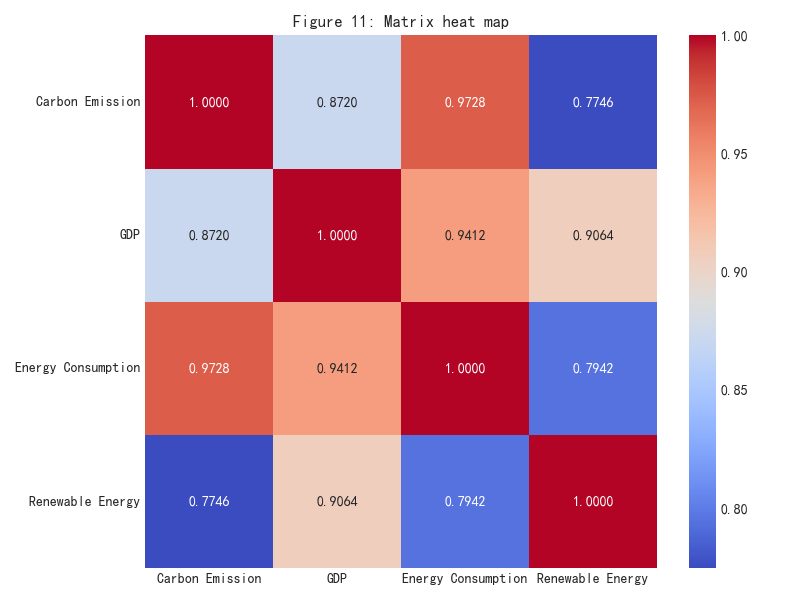
\includegraphics[width=0.8\textwidth]{figure_11_part2.png}
		\caption{Data analysis line chart and matrix heat map.}
	\end{figure}
	\begin{lstlisting}[language=Python]
		def plot_fig11():
		fig, axes = plt.subplots(2, 2, figsize=(12, 10))
		years = np.arange(2010, 2021)
		carbon = [55000, 60000, 65000, 63000, 59000, 62000, 67000, 71000, 73000, 78000, 75000]
		axes[0, 0].plot(years, carbon, marker='o', markersize=4)
		axes[0, 0].set_title('Carbon Emission')
		gdp = [40000, 45000, 50000, 55000, 60000, 65000, 70000, 75000, 80000, 85000, 90000]
		axes[0, 1].plot(years, gdp, marker='o', markersize=4, color='orange')
		axes[0, 1].set_title('GDP')
		energy = [23000, 27000, 28000, 28100, 28000, 29000, 30000, 31000, 32000, 33000, 31500]
		axes[1, 0].plot(years, energy, marker='o', markersize=4, color='green')
		axes[1, 0].set_title('Energy Consumption')
		renewable = [200, 210, 220, 230, 350, 310, 370, 500, 700, 850, 950]
		axes[1, 1].plot(years, renewable, marker='o', markersize=4, color='red')
		axes[1, 1].set_title('Renewable Energy')
		plt.tight_layout()
		plt.savefig('figure_11_part1.png')
		plt.close()
		
		matrix = np.array([[1.0000, 0.8720, 0.9728, 0.7746], [0.8720, 1.0000, 0.9412, 0.9064], [0.9728, 0.9412, 1.0000, 0.7942], [0.7746, 0.9064, 0.7942, 1.0000]])
		labels = ['Carbon Emission', 'GDP', 'Energy Consumption', 'Renewable Energy']
		plt.figure(figsize=(8, 6))
		sns.heatmap(matrix, annot=True, fmt='.4f', cmap='coolwarm', xticklabels=labels, yticklabels=labels)
		plt.title('Figure 11: Matrix heat map')
		plt.tight_layout()
		plt.savefig('figure_11_part2.png')
		plt.close()
	\end{lstlisting}
	
	\subsection{Relational model construction}
	Since within the four indicators, data on GDP and energy consumption for 2023-2060 are known by referring to relevant government documents. Therefore, based on the results of the correlation analysis, a relationship model of new energy power with GDP and energy consumption was constructed. The results are as shown below Table 7:
	
	\begin{table}[H]
		\centering
		\caption{Estimation coefficient table.}
		\resizebox{\textwidth}{!}{
			\begin{tabular}{lcccc}
				\toprule
				Variables & Estimate & SE & t-Statistics & p value \\
				\midrule
				(Intercept) & 557.15 & 828.06 & 0.67284 & 0.52001 \\
				x1 & 0.022264 & 0.0064502 & 3.4516 & 0.0086744 \\
				x2 & -0.05344 & 0.041763 & -1.2796 & 0.23654 \\
				\bottomrule
			\end{tabular}
		}
	\end{table}
	
	\begin{figure}[H]
		\centering
		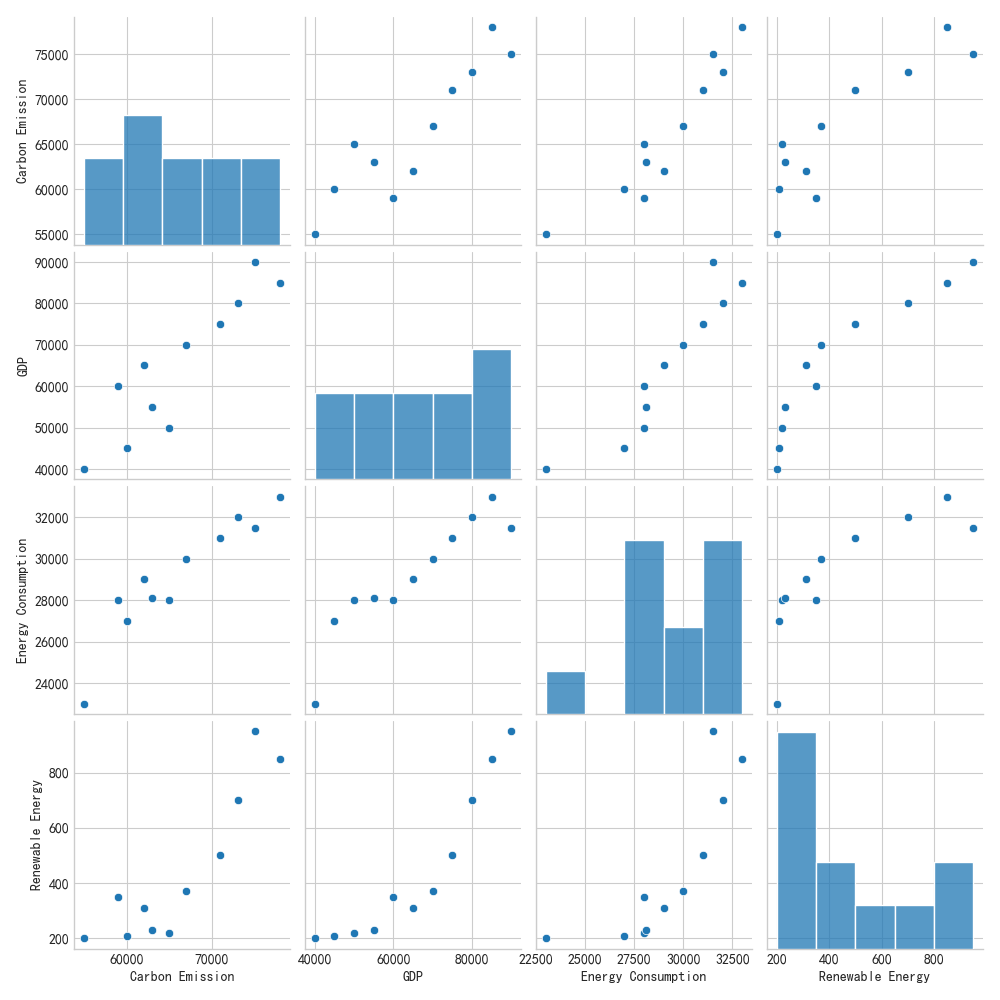
\includegraphics[width=0.8\textwidth]{figure_12.png}
		\caption{Scatter plot matrix.}
	\end{figure}
	\begin{lstlisting}[language=Python]
		def plot_fig12():
		df = pd.DataFrame({'Carbon Emission': [55000, 60000, 65000, 63000, 59000, 62000, 67000, 71000, 73000, 78000, 75000], 'GDP': [40000, 45000, 50000, 55000, 60000, 65000, 70000, 75000, 80000, 85000, 90000], 'Energy Consumption': [23000, 27000, 28000, 28100, 28000, 29000, 30000, 31000, 32000, 33000, 31500], 'Renewable Energy': [200, 210, 220, 230, 350, 310, 370, 500, 700, 850, 950]})
		sns.pairplot(df)
		plt.suptitle('Figure 12: Scatter plot matrix', y=1.02)
		plt.savefig('figure_12.png')
		plt.close()
	\end{lstlisting}
	
	\begin{table}[H]
		\centering
		\caption{Estimation coefficient table.}
		\resizebox{\textwidth}{!}{
			\begin{tabular}{lcccc}
				\toprule
				Variables & Estimate & SE & t-Statistics & p value \\
				\midrule
				(Intercept) & -4298.5 & 4531.4 & -0.94859 & 0.37442 \\
				GDP & -0.29049 & 0.054178 & -5.3618 & 0.0010507 \\
				Energy Consumption & 3.0059 & 0.24403 & 12.318 & 5.3345e-06 \\
				Renewable\_Energy & 7.908 & 1.8822 & 4.2014 & 0.0040286 \\
				\bottomrule
			\end{tabular}
		}
	\end{table}
	
	\subsection{Projections of carbon emissions without photovoltaic power generation}
	Establish models of correlations between carbon emissions and population, GDP, and energy consumption. A linear regression model was established based on the processed data and solved by SPSSPRO, and the results are shown in Table 9.
	
	\begin{table}[H]
		\centering
		\caption{Results of linear regression.}
		\resizebox{\textwidth}{!}{
			\begin{tabular}{lcccccc}
				\toprule
				Variables & Unstandardized B & Standard error & Standardized Beta & t & P & VIF \\
				\midrule
				Constant & 30996.85 & 123996.548 &  & 0.250 & 0.809 &  \\
				Population & -18.798 & 4.653 & -0.778 & -4.040 & 0.005 & 23.384 \\
				Gross domestic product & -0.017 & 0.043 & -0.058 & -0.409 & 0.695 & 12.813 \\
				Total energy consumption & 3.453 & 0.314 & 1.781 & 10.997 & 0.000 & 16.536 \\
				\bottomrule
			\end{tabular}
		}
	\end{table}
	
	The formula for the ridge regression coefficients $\hat{\beta}_{ridge}$ is given by:
	\begin{equation}
		\hat{\beta}_{ridge}=(X^{T}X+\lambda I_{n})^{-1}X^{T}Y
	\end{equation}
	
	The cost function is:
	\begin{equation}
		J(\beta) = RSS + \lambda \sum_{j=1}^{n}\beta_{j}^{2}
	\end{equation}
	
	\begin{table}[H]
		\centering
		\caption{Results of ridge regression analysis.}
		\resizebox{\textwidth}{!}{
			\begin{tabular}{lccccc}
				\toprule
				K=0.045 & Unstandardized B & Standard error & Standardized Beta & t & P \\
				\midrule
				Constant & 27827.599 & 26866.457 & & 1.036 & 0.335 \\
				Population & -1.987 & 3.83 & -0.082 & -0.519 & 0.620 \\
				Gross domestic product & 0.004 & 0.048 & 0.015 & 0.093 & 0.929 \\
				Total energy consumption & 1.926 & 0.311 & 0.994 & 6.191 & 0.000 \\
				\bottomrule
			\end{tabular}
		}
	\end{table}
	
	\begin{equation}
		y = 27827.599 - 1.987 \times P + 0.004 \times GDP + 1.926 \times E
	\end{equation}
	
	\begin{equation}
		x_{NZi} = 3916.326 + 8.585 x_{NNi} + 0.499 x_{NGi} + 0.281 x_{NYi} + 0.763 x_{NYi} + 2.399 x_{NIH} + 0.778 x_{NPI}
	\end{equation}
	
	\subsection{Data comparison}
	Based on Sections 5.3, 5.4, carbon emission data with or without the influence of new energy power data, in order to draw the visualization results more intuitively, this paper draws a line graph for comparison and analysis. As shown below Figure 13.
	
	\begin{figure}[H]
		\centering
		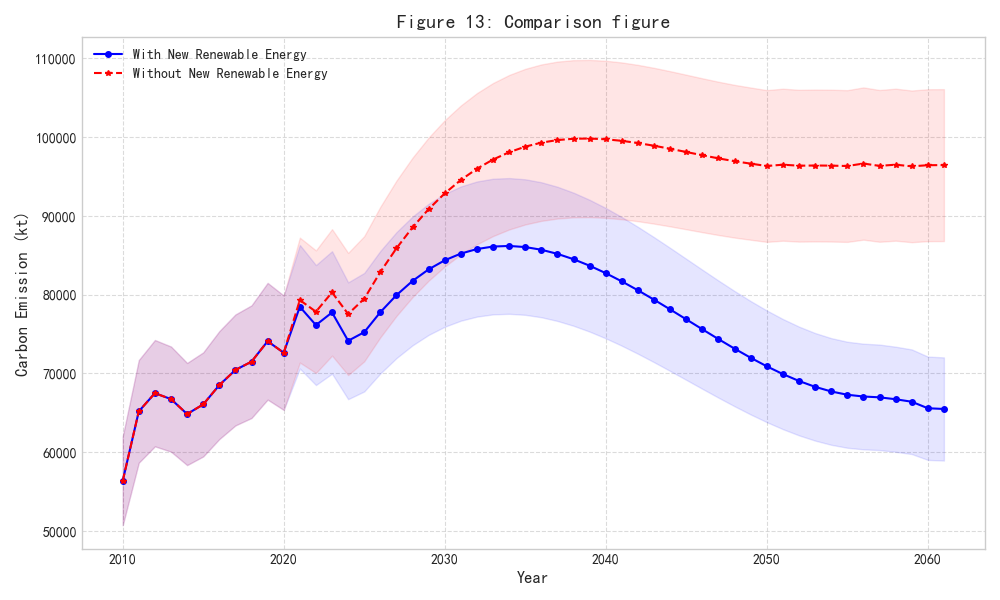
\includegraphics[width=0.8\textwidth]{figure_13.png}
		\caption{Comparison figure.}
	\end{figure}
	\begin{lstlisting}[language=Python]
		def plot_fig13():
		carbon_with = np.array([56360, 65193, 67502, 66749, 64853, 66074, 68526, 70451, 71502, 74096, 72633, 78473, 76147, 77751, 74155, 75245, 77784, 79947, 81753, 83222, 84373, 85227, 85802, 86119, 86196, 86054, 85712, 85190, 84507, 83683, 82738, 81690, 80561, 79368, 78133, 76874, 75611, 74364, 73152, 71995, 70912, 69924, 69049, 68307, 67719, 67302, 67078, 66974, 66731, 66415, 65589, 65496])
		years_15 = np.arange(2010, 2010 + len(carbon_with))
		carbon_without = carbon_with.copy()
		divergence_start = 10
		for i in range(divergence_start, len(carbon_without)):
		gap = (i - divergence_start) * 850 
		carbon_without[i] += gap
		stabilize_idx = 40
		final_val = carbon_without[stabilize_idx]
		for i in range(stabilize_idx, len(carbon_without)):
		carbon_without[i] = final_val + np.random.normal(0, 100) 
		plt.figure(figsize=(10, 6))
		plt.plot(years_15, carbon_with, 'b-o', markersize=4, label='With New Renewable Energy')
		plt.plot(years_15, carbon_without, 'r--*', markersize=4, label='Without New Renewable Energy')
		plt.fill_between(years_15, carbon_with*0.9, carbon_with*1.1, color='blue', alpha=0.1)
		plt.fill_between(years_15, carbon_without*0.9, carbon_without*1.1, color='red', alpha=0.1)
		plt.xlabel('Year', fontsize=12, fontweight='bold')
		plt.ylabel('Carbon Emission (kt)', fontsize=12, fontweight='bold')
		plt.title('Figure 13: Comparison figure', fontsize=14, fontweight='bold')
		plt.legend()
		plt.grid(True, linestyle='--', alpha=0.7)
		plt.tight_layout()
		plt.savefig('figure_13.png')
		plt.close()
	\end{lstlisting}
	
	\section{Conclusion}
	This study systematically analyzed key issues such as power supply forecasting, power station site selection optimization, power generation increase and carbon emission impact of photovoltaic power generation by constructing a multi-dimensional index system and multiple mathematical models. First, based on principal component analysis and particle swarm optimization, a power supply prediction model was constructed to verify the synergy of economic, energy, population and environmental indicators, and to improve data reliability through dimensionality reduction and outlier correction. Secondly, cubic polynomial regression and ridge regression methods were used to predict the trends of power production and carbon emissions from 2024 to 2060. The results showed that the introduction of photovoltaic power generation could significantly reduce the total carbon emissions, verifying its core role in achieving the "dual carbon" goals. The study innovatively combined t-SNE dimensionality reduction with an improved particle swarm optimization algorithm to optimize the efficiency of solving complex nonlinear problems and provide data-driven decision support for regional energy planning.
	
	However, the model has some limitations, primarily its adaptability to policy changes and market fluctuations. The lack of incorporation of dynamic policy factors and multi-source heterogeneous data in the model may affect its prediction accuracy under rapidly changing real-world conditions. Therefore, future studies should focus on integrating these dynamic elements to enhance the model's robustness and predictive power. Incorporating more diverse data sources, such as policy shifts, market behavior, and local or regional conditions, would further improve the model's real-world applicability.
	
	Overall, this study provides a theoretical basis and technical path for the large-scale application and sustainable development of photovoltaic power generation. The model offers significant reference value for promoting the transformation of energy structures, although improvements are necessary to ensure its full adaptability to future challenges.
	
\end{document}